\documentclass[11pt,a4paper]{article}
\usepackage[hyperref]{emnlp-ijcnlp-2019}
\usepackage{times}
\usepackage{latexsym}

\usepackage{url}


%  \usepackage{natbib}
 % \bibliographystyle{plainnat}

\aclfinalcopy % Uncomment this line for the final submission
\pagestyle{plain}

%\setlength\titlebox{5cm}
% You can expand the titlebox if you need extra space
% to show all the authors. Please do not make the titlebox
% smaller than 5cm (the original size); we will check this
% in the camera-ready version and ask you to change it back.

\newcommand\BibTeX{B{\sc ib}\TeX}
\newcommand\confname{EMNLP-IJCNLP 2019}
\newcommand\conforg{SIGDAT}

% Use the lineno option to display guide line numbers if required.

\usepackage{amsmath}
\usepackage{tikz-dependency}
\DeclareMathOperator*{\argmax}{arg\,max}
\DeclareMathOperator*{\argmin}{arg\,min}
\DeclareMathOperator{\E}{\mathop{\mathbb{E}}}

\usepackage{amssymb}% http://ctan.org/pkg/amssymb
\usepackage{pifont}% http://ctan.org/pkg/pifont
\newcommand{\cmark}{\ding{51}}%
\newcommand{\xmark}{\ding{55}}%


\newcommand{\Prob}{\mathbb{P}}%

%\usepackage{pslatex}
%\usepackage{latexsym}
\usepackage[english]{babel}
\usepackage[utf8]{inputenc}
\usepackage{bm}
\usepackage{graphicx}
\usepackage{tikz}
\usepackage{xcolor}
\usepackage{url}
%\usepackage[colorinlistoftodos]{todonotes}
\usepackage{rotating}
\usepackage{multirow}





\usepackage[T1]{fontenc}

\usepackage{pslatex}
%\usepackage{latexsym}
\usepackage[english]{babel}
\usepackage[utf8]{inputenc}
\usepackage{amsmath}
\usepackage{bm}
\usepackage{graphicx}
\usepackage{tikz}
\usepackage{xcolor}
\usepackage{url}
%\usepackage[colorinlistoftodos]{todonotes}
\usepackage{rotating}
%\usepackage{natbib}
\usepackage{amssymb}


\usepackage{amsthm}
 


\newcounter{theorem}
\newtheorem{proposition}[theorem]{Proposition}
\newtheorem{corollary}[theorem]{Corollary}
\newtheorem{question}[theorem]{Question}
\newtheorem{example}[theorem]{Example}
\newtheorem{defin}[theorem]{Definition}
\newtheorem{remark}[theorem]{Remark}
\newtheorem{lemma}[theorem]{Lemma}
\newtheorem{thm}[theorem]{Theorem}


\newcommand{\R}[0]{\mathbb{R}}
\newcommand{\Ff}[0]{\mathcal{F}}
\newcommand{\key}[1]{\textbf{#1}}


\newcommand{\soft}[1]{}
\newcommand{\nopreview}[1]{}
\newcommand\comment[1]{{\color{red}#1}}
\newcommand\mhahn[1]{{\color{red}(#1)}}
\newcommand{\rljf}[1]{{\color{blue}[rljf: #1]}}

\newcommand{\thetad}[0]{{\theta_d}}
\newcommand{\thetal}[0]{{\theta_{LM}}}
\newcommand{\thetap}[0]{{\theta_{P}}}


\title{Theoretical Limitations of Self-Attention in Neural Sequence Models}
\author{Michael Hahn \\ Stanford University \\ mhahn2@stanford.edu}
\date{\today}
\begin{document}
\maketitle
\begin{abstract}
Transformers are emerging as the new workhorse of NLP, showing great success across tasks.
Unlike LSTMs, transformers process input sequences entirely through self-attention.
Previous work has suggested that the computational capabilities of self-attention to process hierarchical structures are limited.
In this work, we mathematically investigate the computational power of self-attention to model formal languages.
Across both soft and hard attention, we show strong theoretical limitations of the computational abilities of self-attention, finding that it cannot model periodic finite-state languages, nor hierarchical structure, unless the number of layers or heads increases with input length.
These limitations seem surprising given the practical success of self-attention and the prominent role assigned to hierarchical structure in linguistics, suggesting that natural language can be approximated well with models that are too weak for the formal languages typically assumed in theoretical linguistics. %limited modeling the formal languages typically assumed in theoretical linguistics.
%Our results precisely describe theoretical limitations of the techniques underlying recent advances in NLP.
\end{abstract}


Transformers are emerging as the new workhorse of NLP; achieving the state-of-the-art in tasks such as language modeling, machine translation, and creating pretrained contextualized word embeddings.
%This poses the question of what kinds of structures they are capable of expressing, and what kinds of computations they are able to perform.
Eschewing recurrent computations, transformers are entirely based on self-attention, performing their computations largely in parallel.
This enables them to scale to very long sequences \cite{vaswani2017attention,dai2019transformer,child2019generating}.
On the other hand, it has been suggested that this limits their expressiveness, as they cannot process input sequentially \cite{tran2018importance,dehghani2018universal,shen2018disan,chen2018best,hao2019modeling}.
One aspect thought to be challenging for sequence models is hierarchical structure and recursion.
Hierarchical structure is widely thought to be essential to modeling natural language, in particular its syntax~\cite{everaert2015structures}.
Consequently, many researchers have studied the capability of recurrent neural network models to capture context-free languages (e.g., \citet{kalinke1998computation,gers2001lstm,gruning2006stack,weiss2018practical,sennhauser2018evaluating,korsky2019computational}) and linguistic phenomena involving hierarchical structure (e.g., \citet{linzen2016assessing,gulordava2018colorless}).
Some experimental evidence suggests that transformers might not be as strong as LSTMs at modeling hierarchical structure~\cite{tran2018importance}, though analysis studies have shown that transformer-based models encode a good amount of syntactic knowledge (e.g., \citet{clark2019bert,lin2019open,tenney2019bert}).

In this work, we examine these questions from a theoretical perspective, asking whether models entirely based on self-attention are theoretically capable of modeling hierarchical structures involving unbounded recursion.
Formally, we study their ability to perform two computations that are thought to be essential to hierarchical structure:
First, their ability to correctly \key{close brackets}, a basic problem underlying all nonregular context-free languages and formalized by the \key{\textsc{Dyck}} language \cite{chomsky1963algebraic}.
Second, their ability to \key{evaluate iterated negation}, which is a basic component of the task of evaluating logical formulas, and which amounts to evaluating the \key{\textsc{Parity}} of bitstrings.
We show that neither of these problems can be solved by transformers and similar models relying entirely on self-attention, unless the number of layers or parameters increases with the input length.
Besides representing basic building blocks of hierarchical structure, these languages also represent large classes of regular and context-free languages, meaning that our results will carry over to wide classes of other formal languages.
Our results therefore also yield more generally limitations on the ability of self-attention to model finite-state languages and context-free languages.
%Our results entail show strong theoretical limitations of self-attention:
%Transformers essentially cannot model non-counter-free regular languages or languages containing unbounded recursion.

%Given the practical success of transformers, these theoretical limitations suggest that natural language can be modeled 

While theoretical studies have investigated the power of recurrent neural network models in depth (e.g., \citet{siegelman1991neural, bengio1994learning, weiss2018practical, miller2018recurrent, merrill2019sequential,korsky2019computational}), the theoretical study of self-attention has begun only recently \citep{perez2019turing}.
%While computational limitations of transformers have been conjectured to exist~\cite{dehghani2018universal}, 
Our study provides the first theoretical results about limitations in the power of transformers.

After discussing related work (Section~\ref{sec:related}), we first introduce self-attention (Section~\ref{sec:def-selfatt}) and two fundamental formal languages representing regular and context-free languages (Section~\ref{sec:langs}).
We then prove that self-attention cannot model these languages using either hard (Section~\ref{sec:hard}) or soft (Section~\ref{sec:soft}) attention.
Finally, we discuss our results (Section~\ref{sec:discussion}).

\section{Related Work}\label{sec:related}
\paragraph{Prior Work on Self-Attention}
Transformers were proposed by \citet{vaswani2017attention}, previous related work using self-attention includes \citet{cheng2016long,parikh2016decomposable,paulus2017deep,lin2017structured}.
It has been a recurrent suggestion in the literature that transformers, relying entirely on self-attention, are restricted computationally, as they cannot process their input sequentially.
\citet{dehghani2018universal} suggested that %transformers are restricted computationally, motivating their proposal of a variant with adaptive and unbounded number of layers.
%They argued that
transformers cannot compute functions that require sequential processing of input, without providing further details or proofs.
Similarly, \citet{shen2018disan,chen2018best,hao2019modeling} have introduced extensions of transformers with recurrence, citing similar intuitions about limitations of transformers.
Our results provide the first explicit formalization of these limitations.

Other studies have experimentally tested the abilities of transformers to learn structures.
Most related to our work, \citet{tran2018importance} compared the ability of transformers and LSTMs to learn hierarchical structure, specifically English subject-verb agreeement and evaluating logical formulas.
Based on their experimental results, they suggested that LSTMs are better at learning hierarchical structure.

\citet{yang2019assessing} experimentally investigated the power of self-attention to extract word order information, finding differences between recurrent and self-attention models; however, these were modulated by the training objective.
\citet{lin2019open} and \citet{tenney2019bert} show that BERT \cite{devlin2018bert} encodes syntactic information.

Theoretical study of transformers was initiated by \citet{perez2019turing}, who theoretically studied the ability of Seq2Seq transformers to emulate the computation of Turing machines.
%There is no contrast between their results and ours:
While we consider incremental modeling of sequences, where the number of computation steps is bounded by the input length $n$, they study the setting in which the transformer computes an unbounded number of autoregressive decoding steps, not bounded in the input length $n$.


\paragraph{Investigating the Power of Sequence Modeling Architectures}
The computational power of recurrent neural networks has been a focus of study.
A particular focus has been on their ability to learn non-regular context-free languages, often thought to provide simple models of recursion and hierarchical structure as found in natural language.

A range of studies has experimentally examined the ability of recurrent networks to model counter languages such as $a^nb^n$ \cite{kalinke1998computation,gers2001lstm,cartling2008implicit,weiss2018practical,suzgun2019evaluating}.
Other work has experimentally studied the performance of reccurent architectures on learning to recognize well-bracketed strings, a similar but more challenging problem \cite{sennhauser2018evaluating,skachkova2018closing,bernardy2018can}.
Beyond modeling formal languages, another line of work has studied the ability of LSTMs to model hierarchical structure as occurring in realistic natural language data \cite{linzen2016assessing,gulordava2018colorless}.

Recently, \citet{merrill2019sequential} and \citet{korsky2019computational} theoretically studied several types of recurrent networks. \citet{merrill2019sequential} showed that -- in the finite precision setting -- LSTMs recognize a subset of the counter languages, whereas GRUs and simple RNNs recognize regular languages.
\citet{korsky2019computational} showed, among other results, that arbitrary-precision RNNs can emulate pushdown automata, and can therefore recognize all deterministic context-free languages.
%Inter alia, their results entail that LSTMs cannot model the multi-symbol Dyck language in the finite precision setting.


A related, though different, strand of research has investigated the power of neural networks to model Turing machines.
A classical result~\cite{siegelman1991neural} states that -- given unlimited computation time -- recurrent networks can emulate the computation of Turing machines.
Very recently, \citet{perez2019turing} have shown the same result for both (argmax-attention) Transformers and Neural GPUs.
The crucial difference between these studies and studies of language recognition is that, in these studies, the networks are allowed to perform unbounded recurrent computations, arbitrarily longer than the input length.

\section{Self-Attention}\label{sec:def-selfatt}
Here we define self-attention as used in Transformers, following \citet{vaswani2017attention}.
We have an input ${\bf x} = x_1 \dots x_n$, where all $x_i$ come from some finite alphabet $\mathcal{V}$, and $x_n$ is an end-of-sequence symbol.
This input is then encoded into a sequence of input embeddings $v_1,\dots,v_n$ using some embedding map $\mathcal{V} \rightarrow \mathbb{R}^k$. %, where $v_i \in \mathbb{R}^k$ are input embeddings, and we assume that $x_n$ encodes an end-of-sequence symbol.
We furthermore have a sequence $p_1, p_2, \dots$ of positional embeddings $p_i \in \mathbb{R}^k$. These are independent of the input ${\bf x}$, and can be computed through some predefined scheme, or could be learned for each position occurring in the training data \citep{vaswani2017attention}.
Input and positional embeddings are combined (e.g., addition or concatenation) to vectors $y_i^{(0)} = f(v_i, p_i)$ ($i=1, \dots, n$), which we will refer to as Layer 0.

A transformer has a fixed number $L$ of \key{layers}; the \key{activations} $y_i^{(k)}$ at position $i$ of the $k$-th layer ($k=1, \dots, L$) are defined as follows.
Each layer has a set of $H$ \key{attention heads}; we first compute attention scores for the $h$-th head:
\begin{equation}
    a_{i,j}^{(k,h)} = f^{att}_{k,h}\left(y_i^{(k-1)}, y_j^{(k-1)}\right)
\end{equation}
where $f^{att}_{k,h}$ is a function combining the activations from the previous level into an attention score.
In practice, this can be implemented e.g. using dot product or additive attention.
The final activation of the head is computed by weighting according to attention weights:
\begin{equation}
    b_{i,k,h} = \sum_{j=1}^n \hat{a}_{i,j}^{(k,h)} y_j^{(k-1)}
\end{equation}
In the soft attention version,
$$ \hat{a}_{i,\cdot} = \operatorname{softmax}(a_{i,1\dots M_i}) $$
where the limit $M_i$ is $n$ in the \key{non-autoregressive} Transformer, and $i-1$ in the \key{autoregressive} one.
In the autoregressive transformer, we set $\hat{a}_{i,j} = 0$ for $j \geq i$.
This definition reflects the need to mask out future observations when the task is to predict upcoming parts of the input, as in language modeling.
In the hard attention variant \cite{perez2019turing}, we take the actual maximum of attention values instead of softmax:
$\hat{a}_{i,j} = \delta_{j, \argmax_{j' = 1, \dots M_i} a_{i,j'}^{(k,h)}}$.\footnote{This requires an arbitrary choice when there are multiple positions with maximal attention weight; we will assume that the one occurring first in the sequence is chosen. Our analysis would also work under other schemes of resolving ties, such as random selection.}

In both versions of attention, the final activation at each position is then computed as
\begin{equation}
    y_i^{(k)} := f^{act}(y_i^{(k-1)}, b_{i,k,1}, \dots, b_{i,k,H})
\end{equation}
where $f^{act}$ is implemented as a fully-connected feedforward network with a skip-connection \cite{vaswani2017attention}.

\paragraph{Hard and Soft Attention}
There is a choice between soft attention and hard attention \cite{shen2018reinforced,perez2019turing}.
The one prior theoretical study of transformers~\cite{perez2019turing} assumes hard attention.
In practice, soft attention is easier to train with gradient descent methods; however, analysis studies suggest that attention often concentrates on one or a few positions in trained transformer models \cite{voita2019analyzing,clark2019bert} and that the most important heads tend to be those that clearly focus on a few positions~\cite{voita2019analyzing}, suggesting that attention often behaves  like hard attention in practice. %, and analysis of neural network attention focuses on the positions where attention concentrates
We will  examine both hard (Section~\ref{sec:hard}) and soft (Section~\ref{sec:soft}) attention settings.
%We will see that, if arbitrary activation functions are allowed, soft attention is significantly more powerful than hard attention.
%On the other hand, in the realistic setting where activation functions obey reasonable regularity conditions (satisfied by ReLU, Tanh, \dots), hard and soft attention result in similar limitations.


\paragraph{Formalizing Language Model and Recognition}
How do we formalize the concept that a Transformer model can accurately model a formal language?
In work on LSTMs, the tasks of language modeling \citep{skachkova2018closing} and recognition \citep{weiss2018practical} have been proposed.
These correspond to the NLP tasks of language modeling and text classification.

\key{Language Modeling} uses the autoregressive variant; here, the activations $y_{i}^{(L)}$ are fed through a linear or feedforward network and a softmax layer that computes a probability distribution $p_i(v)$ over the elements $v$ of the input vocabulary $\mathcal{V}$, attempting to predict the input $x_i$.
Due to the construction of the attention weights $\hat{a}_{i,j}$, the activations $y_{i}^{(L)}$ only depend on input symbols $x_1, \dots, x_{i-1}$, so that $p_i(v)$ computes a distribution that is conditioned only on those preceding inputs: $p_i(x_i|x_1\dots x_{i-1})$.
The \key{cross-entropy} of an autoregressive language model on a distribution over input sequences ${\bf x} = x_1, \dots, x_{|{\bf x}|}$ is $- \mathbb{E}_{{\bf x}} \left[\frac{1}{|{\bf x}|} \sum_{i=1,\dots |{\bf x}|} \log p_i(x_i|x_1\dots x_{i-1})\right]$.
This quantity is minimized if the transformer exactly captures the distribution over input strings.
We will not restrict ourselves to specific input distributions; a natural choice is distributions generated by weighted automata.

%We will mostly consider the uniform distribution over even-parity bit strings of length $n$ for all $n = 1, 2, \dots$ (including an end-of-sequence symbol), where the probability of choosing a length $n$-string is $2^{-n}$.
%Our results hold under any string distribution that hold for any distribution that assigns non-zero probability to each string in the language.



\key{Language Recognition} is the task of classifying input strings as either belonging to (`1') or not belonging to (`0') a formal language~\citep{weiss2018practical}.
%Following~, we formalize this as the sequence-to-sequence task of transducing words to labels $1$ (`in the language') and $0$ (`not in the language').
Following the construction of transformers in sequence-to-sequence tasks \cite{vaswani2017attention}, we compute a softmax probability vector $p(\cdot|{\bf x})$ for this label from the last activation $y_{n}^{(L)}$, obtained after reading the end-of-sequence symbol.
In this task, the transformer can be non-autoregressive.
Here, for some formal language $L$ and a fixed probability distribution over strings, the cross-entropy is $- \mathbb{E}_{{\bf x}} \log p(1_{{\bf x} \in L}|{\bf x})$.
It is zero if and only if the model is correct with perfect confidence on every input.

%While one may think of the uniform distribution as a good example, we will also show results that hold under any string distribution that hold for any distribution that assigns non-zero probability to each string.

%We consider the problem of language recognition as in Weiss et al: a Seq2Seq model is tasked with transducing words in the language to $1$, and other words to $0$.
%To accomodate imprecision in computation, we will relax this to only demand that the result by separated ufrom 0.5 by some constant $\delta$.


%Finite/infinite precision, hardmax/softmax




\section{Regular and Context-Free Languages}\label{sec:langs} % : \textsc{Parity}

We will analyze the ability of transformers to recognize regular and context-free languages, using two prominent representatives (\textsc{Parity} and \textsc{2Dyck}). %, which are basic representatives of wide classes of regular and context-free languages. %; the third (\textsc{LogicalFormulas}) is arguably directly relevant to modeling the meaning of natural language (CITE).
%\textsc{Parity}.


\paragraph{\textsc{Parity}} is the set of bit strings such that the number of $1$s is even.
This is a very simple regular language, recognized by a finite-state automaton with two states.
The regular languages form the lowest layer of the Chomsky hierarchy, and even simple RNNs can compute all regular languages.
Within the regular languages, a particularly basic class is formed by the \emph{counter-free} or \emph{star-free} languages \cite{mcnaughton1971counter}, which can be expressed by regular expressions using only union, complementation, and concatenation.
In some sense, \textsc{Parity} is the simplest non-counter-free, or \emph{periodic}, regular language.
%Any regular language that is not counter-free whose syntactic monoid contains a group are at least computationally as hard as \textsc{Parity}.
This means, if transformers cannot compute \textsc{Parity}, they cannot recognize (almost)\footnote{More precisely, inability to compute \textsc{Parity} entails that they cannot recognize any regular language whose syntactic morphism is not quasi-aperiodic~\cite[p. 488]{barrington1992regular}.} any regular language that is not counter-free.

In the context of natural language, \textsc{Parity} naturally arises in the context of evaluating logical formulas:
%\paragraph{\textsc{LogicalFormulas}} is the set of Boolean formulas evaluating to True. Formally, we consider formulas using binary operators $\wedge, \vee$, negation $\neg$, atomic \textsc{true}, and brackets `(', `)'.
%\cite{tran2018importance} experimentally studied the ability of transformers to learn this language, finding that they did not perform as well as LSTMs.
%\textsc{LogicalFormulas} is also a natural linguistically-relevant setting in which \textsc{Parity} arises:
Evaluating iterated negations is tantamount to counting whether the number of nested negations is even or odd.
If we know that transformers cannot compute parity, this entails that they also cannot evaluate logical formulas accurately.


%For \textsc{Parity}, the language modeling task amounts to predicting well whether the next symbol can possibly be an end-of-sequence symbol -- which is true if and only if the preceding symbols have even parity.


%This contrastsir ability to emulate finite automata is strongly restricted, compared even to simple RNNs.


%Why is \textsc{Parity} interesting?
%The reason is that, as we will show, Parity is a very simple instantiation of certain properties that make a large range of problems hard for parallel computation with a fixed number of layers.
%If transformers cannot compute \textsc{Parity}, it immediately follows that they also cannot compute various more complex functions:




%A system that evaluates logical formulas (CITE) has to (among other things) be able to handle iterated negations.
%
%
%\cite{tran2018importance} experimentally studied the ability of transformers to learn this language, finding that they did not perform as well as LSTMs.


\paragraph{\textsc{2Dyck}} is the language of correctly bracketed words consisting of `(', `[' and `)', `]'.
This language is a very simple model of hierarchical structure.
The Chomsky-Sch{\"u}tzenberger theorem \cite{chomsky1963algebraic} states that any context-free language arises from a variant of \textsc{2Dyck} with multiple types of parentheses through intersection with a regular language and homomorphisms.
Consequently, the ability of LSTMs to model languages such as \textsc{2Dyck} has been an object of experimental study \cite{sennhauser2018evaluating,skachkova2018closing,bernardy2018can}.
%As \textsc{1Dyck} is a deterministic counter language, finite-precision LSTMs are capable of perfectly modeling \textsc{1Dyck};
%Empirically, though they perform less well for versions with multiple types of parentheses \cite{sennhauser2018evaluating}, which are not counter languages any more.
%In contrast, 
Our theoretical results will show that transformers are strongly limited in their ability to model \textsc{2Dyck}, including variants with fewer or more types of parentheses.



%In the case of \textsc{Parity}, we consider the uniform distribution over even-parity bit strings of length $n$ for all $n = 1, 2, \dots$ (including an end-of-sequence symbol), where the probability of choosing a length $n$-string is $2^{-n}$.
%This distribution can be generated by a probabilistic finite automaton with two states.
%In the case of \textsc{2Dyck}, we again consider the uniform distribution, weighted by $2^{-n}$.
%Here, reaching perfect cross-entropy requires classifying both whether the next symbol can be a closing bracket, and which type of bracket would have to be chosen.


%Recognizing whether an expression is bracketed correctly is a basic example of a context-free language and of recursion. If transformers cannot compute parity, they also cannot decide whether long expressions are bracketed correctly.
%To prove this reduction, we first note that a transformer capable of deciding whether an expression is bracketed correctly can be converted into a transformer for deciding whether a string has more $1$s than $0$s. TODO actually not recognizing, but to say whether there can be a closing bracket

%Let a string be given, we then create versions $a'$ and $a''$ where $a'$ has zeroes replaced by some neutral letter, and $a''$ has its ones replaced by that.
%We then concatenate $a'a''$ and interpret zeroes as `(' and ones as `)'.
%This string can be completed to a correctly bracketed one if and only if there are at least as many `('s as there are `)'s.
%Second, we can reduce $Maj_x Maj_y (x\leq y)$ TODO unclear, might explode

%\paragraph{Finite-State Languages with Groups:} 




%\section{Finite Precision}
%We start by examining the case of finite precision.
%We interpret finite precision as meaning that only finitely many floting point numbers are distinguished.\footnote{An alternative interpretation is that numbers can be unboundedly large, but precision is limited, e.g., numbers are only distinguished in intervals of some $\epsilon$.}
%As \cite{perez2019turing} remarked, finite precision means that there are only finitely many distinct positional encodings, and the positions can be partitioned into a finite partition $\mathbb{N} = P_1 \cup \dots \cup P_N$.

%In this case, an input word as processed by the network can be reduced to listing the numbers of 0's and 1's in positions belonging to each of the subsets $P_i$.

%Such a network cannot asymptotically model $a^nb^n$.

%Such a network also cannot model \textsc{Parity}, since the finite-precision activations \dots

%show Parity is not in $Maj_2[un]$: this is actually relatively easy to show, we just have a finite number of bins, and have a numerically imprecise representation of how many are in each bin.

%This argument is quite 

%Finite precision may be an unrealistic assumption for asymptotic analysis:
%If positional embeddings have $d=100$ dimensions, they can robustly distinguish between $2^{100} \approx 10^{30}$ many positions, much more than the input length encountered in any practical NLP application.
%This motivates the study of infinite precision.





\section{Results for Hard Attention}\label{sec:hard}

We will start our analysis with the study of hard attention~\cite{perez2019turing}.
We show that hard attention transformers cannot represent \textsc{Parity} or \textsc{2Dyck}. %, or \textsc{BooleanFormula}.
To keep the results maximally general, our analysis will use combinatorial arguments and make no assumption about, e.g., activation functions and the norms of parameter matrices.
In fact, we do not even assume that the internal position-wise representations $y_{(j)}^k$ in each layer are vector-valued, as opposed to, say, discrete structures.

%\paragraph{General Formalization of Transformers}
%Each head depends on a finite number of activations in the previous layer (skip-connections) and the one argmax thing that was attended to.


%Our results will show that hard-attention transformers are not only unable to recognize these languages perfectly, they are also unable to 




\begin{figure*}[ht]
    \centering
    \begin{tabular}{cccc}
    (a) & (b) & (c) & (d) \\
    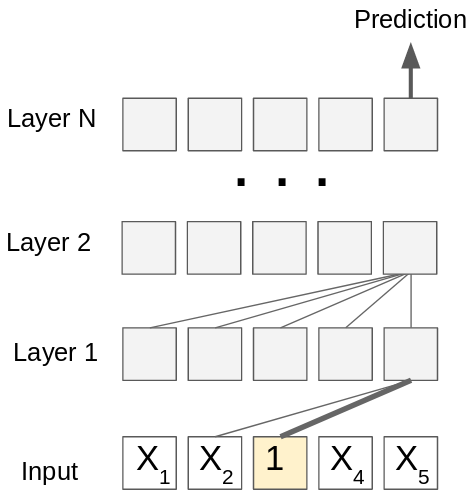
\includegraphics[width=0.23\textwidth]{figures/sa1.png} &
        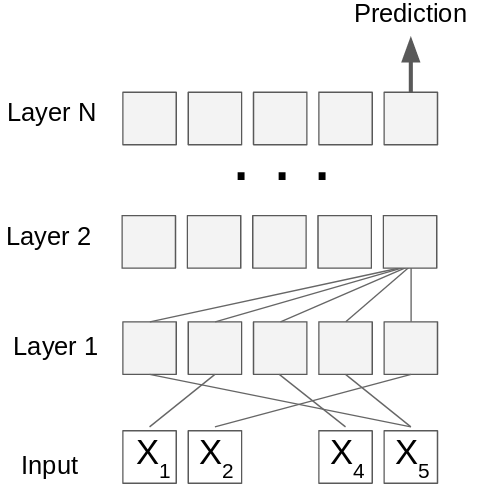
\includegraphics[width=0.23\textwidth]{figures/sa2.png}&
    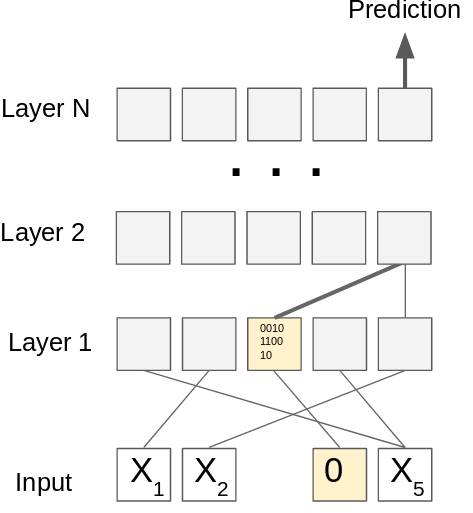
\includegraphics[width=0.22\textwidth]{figures/sa3.png} &
        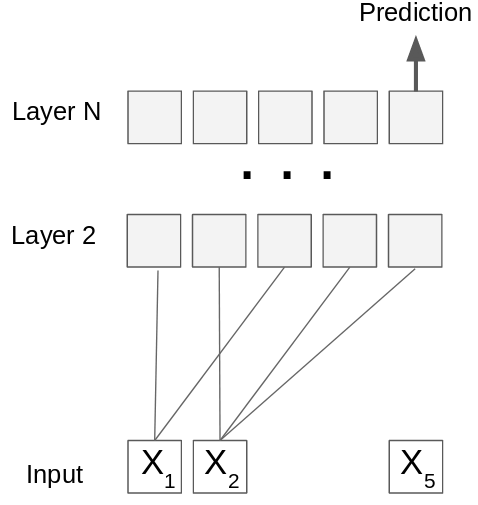
\includegraphics[width=0.23\textwidth]{figures/sa4.png}
        \end{tabular}
	\caption{Iteratively reducing the layers of a transformer by fixing a few input symbols. (a) We fix a small number of input symbols, `attracting' attention from the first layer to a few inputs. (b) After this step, each activation in the first layer only depends on a small number of input symbols. (c) We again fix a few input symbols in such a way as to `attract' attention of layer-1 heads to some layer-0 activations. As a result, each layer-1 activation only depends on a small number of layer-0 activations. (d) After this step, each layer-1 activation only depends on a few inputs, and we can remove layer 1. In this example, input $X_5$ ends up being ignored by the transformer after applying the restriction.}
	\label{fig:depth-reduction}
\end{figure*}


The basic idea (see Figure~\ref{fig:depth-reduction}) behind the proof is that, through fixing a small fraction of the input symbols in a particular way, we can `capture the attention' of the transformer in such a way that it ends up ignoring almost all remaining input symbols.
%More specifically, we will use the following approach.
%We take a transformer, and for each $n$, we consider what happens if we apply this transformer to inputs of that length.
%We show that, for large enough values of $n$, we can find a way to fix a small fraction of the inputs to 0 or 1, such that the prediction of the transformer depends only on a finitely bounded (independently of $n$) number of input positions.
%That is, after fixing these inputs, the transformer ignores a large number of inputs.
This shows that the transformer could not have solved a problem such as \textsc{Parity}, where every single input bit matters.
The idea of using such input restrictions has been successful in the theory of Boolean circuits~\cite{furst1984parity,yao1986separating,hastad1994optimal}.
In particular, \citet{furst1984parity}  famously used it to prove that polynomial-size bounded-depth Boolean circuits with $\wedge, \vee$, and $\neg$ gates cannot compute \textsc{Parity}.
We describe a new method to prove existence of suitable restrictions appropriate to transformers, as the proof approaches from the Boolean circuit literature do not seem to carry over to networks with continuous real-valued activations. %self-attention with unbounded numerical precision. %The proofs have in common the use of the probabilistic method, but the proof method in \cite{furst1984parity} does not appear to generalize to self-attention with infinite precision.


%Notably, our proof will not make any assumption about the nonlinearities, parameter matrices, positional embeddings, etc. -- all that is assumed is the basic self-attention architecture described above.
%We will not even assume that the same parameters are used for different input lengths $n$, only that the number of layers and heads is the same for all $n$.


%(On the other hand, for a problem such as AND or OR, fixing a single input is enough to fix the entire function, and transformers can do these easily indeed)
%\subsection{Preparation}
%We assume that there is only a single head per layer. If there are no restrictions on the number of layers, this is no loss of generality.
%We assume that, if two inputs have the same attention weight, the one with the smaller index is chosen. Our analysis would also work under other schemes of resolving ties, such as random selection.

A \key{restriction} $\rho$ is a family of maps $\rho_n : \{1, \dots, n\} \rightarrow \{*, 0, 1\}$ for $n \in \mathbb{N}$.
A restriction $\rho$ is applied to a transformer by restricting, when the input size is $n$, inputs $x_i$ to the value $\rho_n(i)$ if it is $0$ or $1$.
The output value of the resulting transformer only depends on those inputs $x_i$ such that $\rho_n(i) = *$.

The following technical result formalizes the intuition described above:
\begin{thm}\label{thm:hardmax-main}
Let any transformer be given, and let $C \in (0,1)$.
Then there is a restriction $\rho$ and an integer $c > 0$ such that 
$$|\{i \leq n: \rho_n(i) = *\}| \geq Cn$$
(for all sufficiently large $n$) and such that, on the restricted input, each of the final activations $y_{i}^{(L)}$ depends only on $\leq c$ inputs, independent of input length $n$.
\end{thm}
We first show how this entails that transformers cannot correctly model the two formal languages:
\begin{corollary}
No classifier built from $y_n^{(L)}$ can have perfect accuracy on classifying strings as belonging to \textsc{Parity}, or classifying as belonging to \textsc{2Dyck}.

Therefore, transformers with hard attention cannot model \textsc{Parity} or \textsc{2Dyck} with perfect cross-entropy, for \emph{any} probability distribution that assigns some nonzero probability to every string (classification setting) or to every string in the language (prediction setting). %, or \textsc{BooleanFormula}.
%with cross-entropy asymptotically better than chance.
%, or \textsc{BooleanFormula} (i.e., asymptotic cross-entropy is at chance level).
\end{corollary}
\begin{proof}
Take $C=0.6$.
For \textsc{Parity}, after applying a restriction, the output of the transformer depends on $c$ inputs.
An input of sufficiently large size $n$ thus has unrestricted inputs that do not influence the output.
But flipping a single input bit changes the value, so the transformer's output cannot match membership in \textsc{Parity} beyond chance as soon as $n$ is sufficiently large.
As a consequence, in the prediction task, cross-entropy cannot be perfect as the model cannot reliably identify which prefixes can be followed by the end-of-sequence symbol (namely exactly those prefixes with an even number of ones). 

%As a corollary, transformers also cannot model \textsc{BooleanFormula}, as they cannot model iterated negation.

For \textsc{2Dyck}, we show that hard attention transformers cannot even solve the simpler variant \textsc{1Dyck} with a single bracket type (`(', `)').
We first restrict the first $0.2n$ input positions to `(', and the last $0.2n$ input positions to `)'.
After applying the restriction provided by the theorem, the resulting restricted input will still be compatible with both well-bracketed and non-well-bracketed inputs, but the prediction will depend only on a bounded number of positions.
As the prediction depends on only a bounded number of positions, this shows the transformer could not recognize \textsc{1Dyck}, and thus also not \textsc{2Dyck}.
Again, in the prediction task, the model thus cannot reliably identify when an end-of-sequence symbol is allowed (namely, if and only if the prefix is balanced).
%The probability that 
%for BooleanFormula, maybe the reduction to PARITY is okay, if there is a constant fraction of chance that parity will be relevant
%
%TODO but cross-entropy?
\end{proof}

%\paragraph{Implications for Other Languages}
%As hinted at above, such results about \textsc{Parity} and \textsc{2Dyck} immediately entail results about an extremely wide range of languages.
%The result holds for non-regular context-free languages, subject to a technical condition that limits the usefulness of positional information:
%\begin{corollary}
%The preceding result holds for any language $L$ such that
%\begin{enumerate}
%    \item $L$ is regular and its syntactic morphism is not quasi-aperiodic \citep[p. 488]{barrington1992regular}, or
% $L$ is non-regular and context-free, and there is a non-empty string $e$ such that $xy \in L \Leftrightarrow xey \in L$ for all strings $x,y$.
%\end{enumerate}
%\end{corollary}
%\begin{proof}
%For (1), \cite[p. 488]{barrington1992regular} prove that \textsc{Parity} can be reduced to any such language.
%For (2), we 
%TODO
%\end{proof}




\paragraph{Discussion}
It may be instructive to compare to similar languages that \emph{can} be modeled perfectly by hard-attention transformers.
First, $1^*$ (over the alphabet $\{0,1\}$) is the regular language of words that have only ones and no zeroes; its minimal automaton has two states, like \textsc{Parity}.
A transformer can recognize this by having an attention head that attends to a position with zero input if it exists, and classifies the word as belonging to $1^*$ if and only if none exists.
Second, $a^nb^n$ is a very basic context-free language.
It can be recognized using suitable positional embeddings by (1) having one head attend to the largest position $n$, (2) using this information to attend to any $b$ at position $<n/2$ or any $a$ at position $\geq n/2$. The input belongs to $a^nb^n$ if and only if such a symbol is found.
Very similar reasoning holds in the prediction setting.
A crucial difference between these languages and \textsc{Parity} / \textsc{2Dyck} is that fixing a few inputs can easily force nonmembership, e.g. a single 0 for $1^*$, and an $a$ in the second half for $a^nb^n$.
Therefore, such simple languages are immune to the depth reduction method, and indeed \emph{can} be modeled perfectly with self-attention.


In this context, we note that our depth reduction method applies to languages that are sufficiently `sensitive' in the sense that fixing a constant fraction of input symbols cannot force the word to be inside or outside $L$.
%\begin{corollary}
%Let $L$ be a formal language.
%Assume that, for some $C \in (0,1)$ and for all sufficiently large $n$, fixing at most $C \cdot n$ input symbols cannot force a word to be inside or outside of $L$.
%Then the preceding results hold for $L$.
%\end{corollary}
%\begin{proof}
%Immediate from Theorem~\ref{thm:hardmax-main}.
%\end{proof}
Similar notions of sensitivity of functions %and the structure of Hamming neighborhoods
have been studied in computational complexity~\cite{boppana1997average,gilmer2015new,gopalan2016smooth,rossman2018average} and more recently linked to generalization in feedforward networks~\cite{de2018deep}.
We intend to investigate these connections in future work.

%In general, languages are hard for transformers if any word has $\Omega(n)$ many Hamming neighbor that have the opposite label

%As a corollary, we can show that: (1) Among regular languages, hard-attention transformers can at most model counter-free languages. (2) Among context-free languages that explicitly mark their hierarchical structure through bracketing (such as $a^nb^n$ and \textsc{2Dyck})

\paragraph{Proof Idea of the Theorem}
Our approach for proving Theorem~\ref{thm:hardmax-main} will be to iteratively remove the lowest layer of a given transformer by constructing input restrictions.
This process is illustrated in Figure~\ref{fig:depth-reduction}.
After the first step, each of the heads in the first layer will only depend on a bounded number $c$ of input positions.
In the second step, we apply the same argument to the heads in the second layer, so that each head in the second layer only depends on a bounded number $c'$ of heads in the first layer.
After this step, we can collapse the first layer into a collection of feedforward networks that transform a bounded number $\leq cc'$ of input positions into an activation $y_i^{(0)}$ of the lowest layer.
After this step, the first layer has been entirely removed.
Iterating this argument, we remove all layers until the prediction output only depends on a bounded number of input positions, bounded independently of input length.

After the removal of a layer, the resulting structure is not a transformer any more, as each head in the lowest layer now depends on a \emph{combination} of input positions.
We introduce a technical definition to make this concept precise:

\begin{defin}[$c$-Transformer]
Let $c$ a positive integer. A $c$-transformer of depth $d$ is one in which the layer-0 activations $y_j^0$ depend on the embeddings not just at one position $j$, but are a function of the embeddings at $\leq c$ input positions:
\begin{equation}
    y_j^0 = f^{inp}_{n,j}((x_{i_1^{j,n}}, p_{i_1^{j,n}}), \dots, (x_{i_c^{j},n}, p_{i_c^{j,n}} ))
\end{equation}
Here, the indices $x_{i_s^{j,n}}$ depend on the input length $n$.
\end{defin}

Note that an ordinary transformer  of depth $d$ is also a $1$-transformer of depth $d$.


With this technical notion, we show that we can reduce layers, iteratively removing the lowest layer until no self-attention layer is left:
\begin{lemma}[Depth Reduction Lemma]
Given a $c$-transformer with $d$ layers, and some restriction $\rho$ such that
\begin{equation}
|\{i \leq n: \rho_n(i) = *\}| \geq Cn
\end{equation}
($C \in (0,1]$)
for all sufficiently large $n$.
%with some restriction $\rho^0_n$ already applied, which hits a linear fraction of inputs (TODO clarify how this relates to having more heads).
Choose any $C' < C$.
Then there is a restriction $\rho'$ 
such that
\begin{equation}
|\{i \leq n: \rho'_n(i) = *\}| \geq C'n
\end{equation}
for all sufficiently large $n$, 
and such that the resulting function is computed by a $(H\cdot c\cdot k)$-transformer with $d-1$ layers, for some integer $k$ (depending on $C'$), where $H \geq 1$ is the number of attention heads at each layer and position.
\end{lemma}
Before proving this lemma, we note that it implies Theorem~\ref{thm:hardmax-main}.
\begin{proof}[Proof of Theorem~\ref{thm:hardmax-main}]
%The output of the transformer is determined by the last activations $y_{i}^{(L)}$.
Apply the Depth Reduction Lemma iteratively, choosing the constants $C'$ in the lemma appropriately, until only the zero-th layer remains.
Then, after applying the resulting restriction, the final activation $y_{i}^{(L)}$ is now computed by $y_{i}^{(0)}$, which is determined by a bounded number of input bits.
\end{proof}


%$(ab)^{2n}$ is a regular language with even numbers of a's and b's arranged in a particular order.
%Checking membership amounts to checking that (1) the length is a multiple of four, (2) the symbol is $a$ at odd positions, and $b$ at even positions.
%With suitable positional embeddings, we can construct a transformer that attends to any position violating (2)

%In particular, the resulting $c$-transformer can be rewritten into a $c'$-transformer with one layer removed.

%\begin{proof}
\subsection{Proving the Depth Reduction Lemma}
The rest of this section will be devoted to proving the Depth Reduction Lemma.
We will do the first part of the argument for any integer $k \in \mathbb{N}$.
In the second part, we will select a sufficiently large $k$.
%The aim is that $c' := ck$.

\paragraph{Part 1: Preliminaries}
%For the $i$-th level-1 head, we assemble for all inputs $j$ maximum attention value between head $i$ and input $j$ for the two possible inputs $0$, $1$.
%Then we sort the inputs $j$ in descending order by the maximum attention value: $j_1, j_2, \dots, j_n$ (if there are ties, we order by position).

%The following observation will be important: If we fix the input $j_k$ to the value that makes the attention value achieve the higher value, then the activation at element $i$ in level 1 only depends on the inputs $i, j_1, \dots, j_{k-1}$.

Fixing the input length $n$, we say an input $x_i \in \{x_1, ..., x_n\}$ is $\rho$-\key{free} if $\rho_n(i) = *$.
We construct the restrictions $\rho'_n$ separately for each $n$.
For each layer-1 attention head $h$ at position $i$ and each position $j \in \{1, \dots, n\}$, we compute the maximum possible attention value that can be achieved for this pair:
\begin{equation}
\max_{x_1\dots x_n \text{ compatible with } \rho_n} f^{att}_{k,h}(y_i^{1}, y^{1}_j)
\end{equation}
We order the positions $\{1, \dots, n\}$ downwards by this value, obtaining a sequence $j_1, \dots, j_n$ for each layer-1 attention head $h$ at a position $i$ (In the case of ties, we order by  position). If the Transformer is autoregressive, we order the positions $i, \dots, n$ after the positions $1, \dots, i-1$, irrespective of the attention weights.

For each layer-1 attention head, we then select a sequence $1 \leq i_1 < i_2 < \dots < i_k \leq n$ such that (1) for each $i_s$, there is at least one $\rho$-free input that only feeds into the element $j_{i_s}$ and no other $j_{i_s'}$, (2) $i_k$ is minimal, i.e. there is no subsequence with smaller $i_k$ that also satisfies (1).
There is only one case in which we cannot find such a subsequence, which is if all $j_1, \dots, j_n$ together depend only on $< ck$ $\rho$-free inputs, in which case this head already satisfies the condition we're aiming for.

A layer-1 head $k$-\textbf{depends} on some $\rho$-free input $x_i$ if $\rho_n(i) = *$ and $x_i$ appears as an input to some $j_r$ for $r \leq i_k$.
A layer-1 head $k$-depends on a $\rho$-free input if and only if that input appears as an input to some $j_{i_s}$ ($s \leq k$). (This is since $i_k$ is minimal).

Two layer-1 head are $k$-\textbf{neighbors} if some $j_{i_s}$ for one and $j_{i_s'}$ for the other both $k$-depend on some input $x_l$.

%We first show that, WLOG, we can assume that every layer-1 head has $\leq f = 2c^2k^2H$ many $k$-neighbors.
%We do this by creating a restriction that hits at most a linear fraction of inputs that enforces this.

%So let's assume there are heads with $f > 2c^2k^2H$ many neighbors (we do this argument for all values of $n$).
%Any head only depends on $\leq ck$ many inputs; by the Pigeonhole principle, this means,

We will construct input restrictions using probabilistic arguments over i.i.d. random restrictions.
For this approach to succeed, we require a  sufficient amount of independence between the activations of different heads in layer 1.
We thus need to ensure that the number of $k$-neighbors of each head is bounded.

Fix some $\eta \in (0,1)$ (to be chosen later).

Let $H$ be the number of attention heads in each position of layer 1.
First, assume there is some $\rho$-free input that has $>\frac{1}{\eta}kcH/C$ many $k$-depending layer-1 heads.
%We now show that the number of such inputs is small, and that we can remove those WLOG.
Assume the number of such inputs is larger than $\eta Cn$ for some $n$.
Then, the number of pairs of inputs and depending level-2 heads would be more than $> \eta C n \cdot \frac{1}{\eta} H k c/C = Hckn$ for this $n$.
On the other hand, there are only $\leq Hckn$ many pairs of $\rho$-free inputs and depending layer-1 heads -- contradiction.
Thus, the number of such inputs is at most $\leq \eta Cn$ for all $n$.
We can therefore modify the restriction $\rho_n$ so that they are set to some fixed value (doesn't matter which one) for these $<\eta Cn$ $\rho$-free inputs, and unchanged for the others.
After this manipulation, every $\rho$-free input has at most $\frac{1}{\eta}kcH/C$ many $k$-depending layer-1 heads, independent of $n$.

Furthermore, assume the number of inputs with $> \frac{1}{\eta} c/C$ depending layer-0 activations is $\geq \eta Cn$.
Then the number of pairs of inputs and layer-0 activations is $>\eta Cn \cdot \frac{1}{\eta} c/C = nc$.
But there are at most $nc$ such pairs, contradiction.
So the number of inputs with $> \frac{1}{\eta} c/C$ depending layer-0 heads is $\leq \eta Cn$.
We can again restrict these inputs to some fixed value (again, it doesn't matter which one).

After these preparations, 
\begin{equation}
|\{i \leq n: \rho_n(i) = *\}| \geq (1-\eta)^2 C n
\end{equation}
for all sufficiently large $n$.

%Now consider those layer-1 heads that have $f > 2c^2k^2$ many $k$-neighbors.

%If there are $\leq n/(1.1c)$ many such heads (for some infinite subsequence of $n$'s -- we can throw away the other $n$'s -- for bad $n$'s, we just fix every input, and they'll drop out of the $\limsup$), then we can fix them manually, fixing only $\leq n/1.1$ many inputs. [I don't think we need this case -- the Case A below subsumes this, and doesn't presuppose the existence of many bad elements]

%So there are $> n/(1.1c)$ many such elements with $f > 2c^2k^2$ many neighbors (for all but finitely many $n$ -- we can throw away the other $n$'s).
%By the Pigeonhole principle, this means, there is some input that has $> 2kc$ many $k$-depending layer-1 heads.

%\begin{enumerate}
%\item Case A: the number of inputs with $\leq 2Hkc$ many $k$-depending layer-1-heads is $o(n)$ as $n\rightarrow\infty$, so the number of inputs with $> 2Hkc$ attached layer-1-heads dominates any linear fraction. Then, the number of pairs of inputs and depending level-2 heads would be at least $0.99 \cdot n 2 H k c > Hckn$ for $n$ sufficiently large. On the other hand, there are only $Hckn$ many pairs of inputs and depending level-2 heads.

%\item Case B: The number of inputs without $> 2kcH$ many $k$-depending layer-1-heads is $\Omega(n)$ as $n\rightarrow \infty$, in which case we can just fix these bad inputs (whose complement is asymptotically at least linearly large) to a fixed value. After this manipulation, $f \leq 2k^2c^2H$. We have hit only a linear fraction of inputs; by Remark above, we can rewrite this into a $c$-transformer with a potentially larger number of heads.
%\end{enumerate}

%NOTE:
%The number of pairs between input and level-2 heads is $\leq Hckn$.
%So the number of heads where that have more than $100 Hck$ attached layer-1 heads is $\leq n/100$.
%So we can make the fraction of replaced inputs very small.

%The number of heads that have to be satisfied is now $\leq Cn$, for some $C$ that was determined by the manipulations we made above. (this means that the restriction to one head per $n$ was unnecessary)

\paragraph{Part 2: Constructing Restrictions}
After the previous part, we are in the setting where every input has $\leq \frac{1}{\eta}kcH/C$ many depending layer-1 heads, and consequently every layer-1 head has at most $f \leq \frac{1}{\eta}c^2k^2H/C$ many $k$-neighbors (for any $k$).
%(Note that the transformations carried out above could at most have increased the value of $H$).
Also, every input has $\leq \frac{1}{\eta}c/C$ depending layer-0 heads.

% after applying restrictions $\rho_n$ such that $\limsup_{n\rightarrow\infty} |\{i \leq n: \rho_n(i) = *\}| = +\infty$.
%Note that the previous part works for any $k$; we will choose a suitable $k$ in this section.

In order to prove the existence of suitable input restrictions, we apply the ``probabilistic method'': we define a probability distribution over restrictions $\rho'$ of inputs, and show that the probability mass assigned to restrictions of the type we require is strictly greater than zero, showing that such a restriction exists.

For each input length $n$, define a probability distribution over restrictions,  independently assigning to each $\rho$-free input position $i \in \{1, \dots, n\}$ the symbol $*$ with probability $q \in (0,1)$ (to be chosen later), and $1$ or $0$ with equal probability else.
On those inputs where $\rho_n(i) \neq *$, we require this random restriction to agree with $\rho_n(i)$.
For the $i$-th layer-1 attention head (there are at most $Hn$ many such), define $X_i$ to be the event that, for the $i$-th head, none of $j_{i_1}, \dots, j_{i_k}$ are assigned the value that produces the highest attention weight (each of these is assigned either the other value, or $*$).
Define $X_0$ to be the event that more than $(1+\delta)qCn$ many inputs are set to $0/1$.

We first show that the probability of $X_i$ ($i=1, ..., Hn$) decays exponentially in $k$.
For the $i$-th attention head, let $Y_i^t$ ($t=1,\dots,k$) be the event that the layer-0 activation $j_{i_t}$ is not assigned the value that produces the highest attention weight, for the given attention head $i$.
Note that $X_i = \bigcap_t Y_i^t$.
We have $\Prob(Y_i^s) = 1-(q/2)^c \in (0,1)$. % (where $q = 1-p$).
Any $Y_i^s$ can be statistically dependent on at most $c \cdot \frac{1}{\eta}c/C = \frac{1}{\eta}c^2/C$ other events $Y_i^{s'}$.
Therefore, there is a set of $\geq \frac{k}{\frac{1}{\eta}c^2/C}$ independent events among these.
Call these $Y_i^{t_1}, \dots, Y_i^{\frac{k}{\frac{1}{\eta}c^2/C}}$.
Then $X_i \subseteq \bigcap_{s=1}^{\frac{k}{\frac{1}{\eta}c^2/C}} Y_i^{t_s}$, and thus
\begin{equation}
    \Prob(X_i) \leq \prod_{s=1}^{\frac{k}{\frac{1}{\eta}c^2/C}} P(Y_i^{t_s}) = \left(1-(q/2)^c\right)^{\frac{k}{\frac{1}{\eta}c^2/C}}
\end{equation}
%We use induction over $t \in \{1, \dots, k\}$ to compute the probability that none of $j_{i_1}, \dots, j_{i_t}$ are assigned to value achieving the maximal attention weight.
%At $t=1$, the failure probability for $j_{i_1}$ is $\leq (1-(q/2)^c)$.
%For $t+1$: Assume that $j_{i_{t+1}}$ introduces $w > 0$ new input variables not occurring in $j_{i_1}, \dots, j_{i_1}$.
%Failure probability is $\leq F_t \cdot (1-(q/2)^w)$.
%TODO maybe this isn't actually strict enough
%\end{proof}
Furthermore, a Chernoff bound gives~\cite{mitzenmacherprobability}
%\footnote{See \url{https://en.wikipedia.org/wiki/Chernoff_bound#Multiplicative_form_(relative_error)}}
\begin{equation}
\Prob(X_0) \leq    \exp\left(-\frac{\delta^2qCn}{(2+\delta)}\right)
\end{equation}
since the number of independent multinomial samples in the sampling of $\rho'$ is at least $Cn$.
We want to show that we can find $q \in (0,1)$, $A, B \in (0,1)$ such that the following holds: %, assuming $f \leq $:
\begin{align}
\Prob(X_i) &\leq  D^k \leq A(1-B)(1-A)^{\frac{1}{\eta}c^2k^2H/C} \\
\Prob(X_0) &\leq \exp\left(-\frac{\delta^2qCn}{(2+\delta)}\right)  \leq B (1-A)^{Hn}
\end{align}
where $D =  \left(1-(q/2)^c\right)^{\frac{1}{\frac{1}{\eta}c^2/C}} \in (0,1)$. % is a constant in $(0,1)$, depending on $c$, $q$, $C$, $\eta$, but \emph{not} on $k$.
Once we have shown this, then by the asymmetric Lov{\'a}sz Local Lemma \cite{mitzenmacherprobability}, there is some input restriction that avoids all events $X_0, X_1, X_2, \dots$.

Choose %$q=0.5$, $\delta=0.5$, 
$A=\frac{1}{k^2}$, $B=0.5$.
First, we need to satisfy
\begin{align}
    D &\leq A^{1/k}(1-B)^{1/k}(1-A)^{\frac{1}{\eta}kc^2H/C} 
\end{align}
For the RHS, 
\begin{equation}
\lim_{k\rightarrow \infty} A^{1/k} = \lim_{k\rightarrow \infty} \exp\left(-\frac{\log k^2}{k}\right) = 1
\end{equation}
Also, $\lim_{k\rightarrow \infty} (1-A)^{\frac{1}{\eta}kc^2H/C}$ equals
\begin{equation}
\lim_{k\rightarrow \infty} \left(1-\frac{1}{k^2}\right)^{Ek} = \lim_{k\rightarrow \infty} \left(1-\frac{E^2}{k^2}\right)^{k} = 1
\end{equation}
where we choose $E = \frac{1}{\eta}c^2H/C$. So, if we choose $k$ large enough (independently of $n$), the RHS can be made arbitrarily close to $1$, in particular, greater than the LHS.

In order to also satisfy
\begin{equation}
\exp\left(-\frac{\delta^2qC}{(2+\delta)}\right)  \leq B^{1/n} (1-A)^H
\end{equation}
make $n$, $k$ large enough to satisfy the inequality (again, choosing $k$ independent of $n$). %so large that $B^{1/n} > 0.99$ and $(1-A)^H = (1-\frac{1}{2k^2c^2})^H > 0.99$.
In conclusion, there exists, for each sufficiently-large $n$, a restriction $\rho'_n$ that avoids all events $X_0, X_1, X_2, \dots$.

With such a $\rho'$, $|\{i \leq n: \rho_n'(i) = *\}|$ is at least
\begin{equation}
\geq (1-\eta)^2\cdot (1-(1+\delta)q) C n
\end{equation}
for all sufficiently large $n$.
Then choose $\eta \in (0,1)$ small, $q \in (0,1)$ small, and $\delta >0$ (such that $(1+\delta)q \in (0,1)$) in such a way to achieve $(1-\eta)^2\cdot (1-(1+\delta)q) = C'/C$.



%Consider $A=2^{-a}$.
%So $2^{-a/k} (1-2^{-a})^{2kc^2} = 2^{-a/k} (\sum_{j=1}^a 2^{-j})^{2kc^2} = (\sum_{j=1}^a 2^{-j-a/{2k^2c^2}})^{2kc^2}$. After we have fixed $k$, we can adjust $a$ to make $a/{2k^2c^2}$ as small as desired to make the result be close to $1$.
%\end{proof}

We now note that, since every layer-1 head depends only on $\leq ck$ many inputs after applying $\rho'$, each layer-1 activation $y_j^{(1)}$ only depends on $\leq Hck$ many inputs.
We can thus collapse layers 0 and 1, converting layer-1 activations into layer-0 activations $y_j^{(0)}$, and obtain a $(Hck)$-transformer performing the same computation as before when $\rho'$ is applied.
This concludes the proof of the Depth Reduction Lemma.


%Can the same proof work for Dyck? Fix the first $0.2n$ to `(', and can we force the random restrictions to only restrict $0.3n$ (replace $2$ by $10$)?




\section{Results for Soft Attention}\label{sec:soft}

%We first notice that, with arbitary activation functions, infinite precision softmax transformers:
%For simplicity, we consider languages over alphabets with only two elements, though the argument generalizes.
%Take positional embeddings $p_i = 2^{-i}$; and set $y_i^0$ to be $p_i$ if $x_i$ is $1$, and $0$ else.
%Then, by using an attention head that attends to each position with equal weight, we can compute $\frac{1}{n} \sum_{i : x_i = 1} 2^{-i}$.
%TODO

%In an actual transformer, all operations are Lipschitz.
%If we use additive attention, 
%If the norm of positional and input embeddings is bounded as $\|p_i\|_2, \|x_i\|_2 \leq p$, 
%The norm of activations in layer $k$ is bounded as $L^k p$.

In the previous section, we showed that transformers using hard attention are not able to recognize a range of core formal languages.
In this section, we study soft attention.
It turns out that proving limitations as strong as what we found in the hard attention setting would settle a major open problem in computational complexity, and might therefore be hard to attain with currently available mathematical methods.\footnote{Showing that soft attention transformers cannot achieve perfect accuracy on evaluating Boolean formulas would separate the complexity classes $LTC^0$ and $NC^1$, a widely conjectured but long-open problem in computational complexity.}
Nonetheless, we will be able to prove similar limitations in this setting, by showing limitations on the  achievable \emph{perplexity}.
Here, we will use the smoothness of the operations used in transformers to show that any transformer, as inputs get longer, will not be able to robustly separate members of the languages from other inputs.
The idea behind the proof is that the impact of any single input on the output of the transformer is small if the input is long:
\begin{lemma}\label{lemma:diff-1n}
If we exchange one input symbol, %a single input bit $x_i$ with the bit $x_i'$
%then the change in the resulting activations at the decoder layers is bounded as $\mathcal{O}(\frac{1}{n})$ with constants depending on the parameter matrices, where $n$ is the input length. %, $k$ is the number of layers, and $C$ is the summed norm of the parameter matrices.
then the change in the resulting activations $y_i^{(L)}$ is $\mathcal{O}(\frac{1}{i})$ in the autoregressive case and  $\mathcal{O}(\frac{1}{n})$ in the non-autoregressive case, for all $i = 1, \dots, n$ except the one at which the change was made, with constants depending on the parameter matrices (independently of $i$ or the input length).
\end{lemma}
This contrasts with recurrent networks:
Changing a single input can have nonnegligible impact on the final state even for very long input.
E.g., an RNN recognizing \textsc{Parity} through a hidden state that encodes parity of the current prefix will flip its hidden state in all future time steps if a single input bit is flipped.


This result entails that, as inputs become longer, soft attention transformers cannot robustly model the two formal languages:
%To make this precise, we take a more quantitative angle and assign probability distributions over inputs for each input length $n$, and consider the behavior of cross-entropy as $n\rightarrow\infty$.
%For \textsc{Parity}, we simply consider the distribution over i.i.d. bitstrings of length $n$, and consider the task of predicting whether the next symbol can be the \textsc{EndOfSequence} symbol -- which is true if and only if the prefix has an even number of ones. % the label (odd or even) from the string.
%For \textsc{LogicalFormulas}, we consider the uniform distribution over formulas of length $n$, again considering the task of predicting the label (TRUE or FALSE).
%For \textsc{2Dyck}, we take the uniform distribution of well-bracketed prefixes of length $n$, and ask the model to classify the set of valid next characters, which is a subset of $\{(,),[, ]\}$.\footnote{Only an exponentially small subset of the strings over $n$ symbols are well-labeled; thus, cross-entropy on the classification task is less meaningful for this language. Considering prediction of the next symbol sidesteps this issue.}
%We consider the problem of predicting the label from the input separately for each input length $n$, and consider cross-entropy as $n\rightarrow \infty$.

\begin{thm}
Let a soft attention transformer be given for one of the languages \textsc{Parity} and \textsc{2Dyck}. %, \textsc{BooleanFormula}.

In the prediction task, as $n\rightarrow\infty$, cross-entropy converges to unigram chance level.

Consequently, the transformer cannot achieve perfect cross-entropy on either the prediction or recognition tasks.
\end{thm}

\begin{proof}
For \textsc{Parity}, exchanging a single bit flips membership.
Thus, for any member of the language, there is an equally likely non-member such that the output activations differ by
only $\mathcal{O}(\frac{1}{i})$.

For \textsc{2Dyck}, the probability that a well-bracketed prefix of length $n$ is exactly balanced is $o(1)$.
In all other cases, the correct label includes one of the two closing parentheses, which depends on one single previous symbol, and both possibilities are equally likely if that symbol is unknown.
%For \textsc{BooleanFormula}, 
\end{proof}

\subsection{Proof of the Lemma}
Having established the main theorem, we proceed to proving the technical Lemma~\ref{lemma:diff-1n}:
\begin{proof}[Proof of Lemma]
We only need to prove the lemma in the non-autoregressive case.
The autoregressive case follows by considering the prefix $x_1, ..., x_i$ up to the given position $i$ as the input.

Let us compare the activations at the decoder layer for two inputs that only differ in the input at the $i$-th position.
Let $D = \|x_i-x_i'\|_2$ the norm of the difference of the input embeddings at this position.

	We show by induction over $k$ that, for some some $C > 0$ (depending on the parameter matrices) the difference between the activations $y_j^k$, ${y_j^k}'$ are bounded as: %at this position are bounded independently of input length $n$:
\begin{equation}
\begin{aligned}
	\|y_i^k-{y_i^k}'\| &\leq (2C)^{2k}D = \mathcal{O}(1) \\
	\|y_j^k-{y_j^k}'\| &\leq \frac{H^k (2C)^{2k}D}{n} = \mathcal{O}(1/n)\ \ \ (j \neq i)
	\end{aligned}
\end{equation}
Once we have shown this, we have found that the influence of any individual input on the final prediction is $\mathcal{O}(\frac{1}{n})$, with constants depending on the norms of parameter matrices and the number of layers.


For $k=0$, $\|y_i^0 - {y_i^0}'\| \leq D$,\footnote{We are assuming that $f$ is addition or concatenation \cite{vaswani2017attention}; for operations such as an MLP, there would be an additional Lipschitz constant depending on parameters and activation functions.}
and %, where $L_f$ is the Lipschitz constant of the operation $f$ combining position and input embeddings.
$\|y_j^0 - {y_j^0}'\| = 0$ for $j \neq i$.

For $k>0$, we first note that for activations $\|y_i^k\|_2 \leq 2 \left(L_{f^{act}}\right)^{L}  (\|p_i\| + \|x_i\|) =: F$, where
$L_{f^{act}}$ is the Lipschitz constant of $f^{act}$.
As $f^{act}$ is implemented as a ReLU MLP \cite{vaswani2017attention}, $L_{f^{act}}$ depends on the norms of the parameter matrices.
Attention logits are bounded by $A := F^2 L_{f^{att}}$ in the case of multiplicative/bilinear attention, and $A := 2 F L_{f^{att}}$ in the case of additive attention.
%If attention logits are bounded as $|a_i| \leq A$,
Then any attention weight $\widehat{a}_{j,i} = \exp(a_i)/\sum_j \exp(a_j)$ is upper bounded by $\frac{\exp(A)}{\exp(A) + (n-1) \exp(-A)} \leq \frac{\exp(2A)}{n}$.

Choose $C : = 2(1 + \exp(2A) + L_{f^{act}})$.

Recall $y_i^k := f^{act}(y_i^{k-1}, b_{i,k,1}, \dots, b_{i,k,H})$, where $b_{i,k,h} = \sum_{j=1}^n \hat{a}_{i,j}^{k,h} y_j^{k-1}$.
We first calculate
\begin{align*}
& \|b_{j,k,h} - b_{j,k,h}'\|  \leq \sum_{w=1}^n \hat{a}_{j,w}^{k,h} \|y_w^{k-1} - y_w^{k-1}\| \\
& \leq + \hat{a}_{j,i}^{k,h} \|y_i^{k-1} - y_i^{k-1}\|  + \sum_{w \neq i} \hat{a}_{j,w}^{k,h} \|y_w^{k-1} - y_w^{k-1}\|  \\
& \leq \frac{\exp(2A)}{n}  (2C)^{2(k-1)} D + \frac{H^{k-1}(2C)^{2(k-1)}D}{n} \\
%& \leq (2C)^{2(k-1)}D \frac{C/2   + H^{k-1} }{n} \\
& \leq \frac{H^{k-1} (2C)^{2(k-1)+1} D}{n}
\end{align*}
Then, $\|y_j^k - {y_j^k}\|$ is at most
\begin{equation}
	L_{f^{act}} \cdot \left(\|y_j^{k-1}-{y_j^{k-1}}'\| + \sum_{q=1}^H \|b_{i,k,q} - b_{i,k,q}'\|\right)
\end{equation}
If $j= i$, this is bounded (as $n \rightarrow \infty$)
\begin{equation}
\leq L_{f^{act}} \cdot ((2C)^{2(k-1)}D + o(1)) \leq (2C)^{2k}D
\end{equation}
If $j\neq i$, this is bounded above by
\begin{align*}
  &  L_{f^{act}} \cdot \frac{H^{k-1} (2C)^{2(k-1)}D + H^{k} (2C)^{2(k-1)+1} D)}{n} \\
  &  \leq  \frac{H^{k} (2C)^{2k} D}{n} \\
\end{align*} 
This proves the inductive step for $k>0$.
\end{proof}


%This shows that, as inputs get arbitrarily long, a soft attention transformer cannot robustly respond to small changes in the input.
%This result stands in marked contrast to recurrent networks, where the impact of individual inputs on the final activation does not in general decay with sequence length.
%In practice, we predict that soft attention transformers will need more layers and larger parameter values to solve formal languages like \textsc{Parity} on longer and longer inputs.
%show the perplexity thing:
%If the attention activations are bounded in norm by $L$ (which comes from the norms of the parameter matrices), then attention will ultimately be swamped, and asymptotically no individual element can have nonnegligible impact.
%Here should have some experimental things


%\footnote{This result appears to contradict the claim in \cite{merrill2019sequential} that softmax asymptotically turns into the average of the attentions attended to most strongly. Our result shows that this would require }




\section{Discussion}\label{sec:discussion}

We have shown that, even with infinite precision, transformers cannot robustly model non-counter-free regular languages, nor basic hierarchical structure.

How do our results compare to what is known about LSTMs?
Recurrent networks such as SRNNs and LSTMs can perfectly emulate finite-state automata, and therefore can model any finite state language with optimal cross-entropy, as long as the state transition and symbol emission distributions are Markovian.
In particular, \textsc{Parity} of i.i.d. bitstrings can be classified with zero cross-entropy, independent of the input length.

Infinite-precision RNNs and LSTMs can model stacks \cite{tabor2000fractal,gruning2006stack,kirov2012processing,korsky2019computational} and thus are theoretically capable of modeling \textsc{2Dyck} and other deterministic context-free languages at optimal cross-entropy and perfect classification accuracy. % and \textsc{LogicalFormulas} perfectly.
This clear contrast between infinite-precision LSTMs and our findings for infinite-precision transformers may provide a theoretical explanation for the empirical finding that LSTMs seem to outperform transformers in modeling hierarchical structure \citep{tran2018importance}.
%On the other hand, the theoretical results of \cite{merrill2019sequential} show that finite-precision LSTMs cannot model these languages perfectly at long lengths.
%Experimental evidence on the ability of LSTMs to learn \textsc{2Dyck} and \textsc{LogicalFormulas} from data is mixed, but clearly falls short of perfect accuracy or cross-entropy.


%In the setting of RNNs and LSTMs, some prior studies have considered the impact of finite numerical precision~\cite{weiss2018practical, merrill2019sequential, korsky2019computational}.

%It is important to remark that all our impossibility results require taking large inputs:
%Certainly, for any bound on the input length, we can construct a transformer that does anything we want.
%However, we are interested in the extent to which a transformer is able to handle arbitrarily long inputs -- similar to analogous work on RNNs/LSTMs/GRUs.

%Our results are consistent with the fact that transformer-based models tend to have far more layers than comparable LSTMs (CITE).

Hierarchical structure, at least at the level of context-free languages, is widely thought to be essential to modeling the structure~\cite{everaert2015structures} and meaning~\cite{montague1973proper} of natural language.
Our results entail that self-attention is strongly limited in its ability to model context-free languages or evaluate logical formulas.
How should we reconcile this with the success of transformers at many natural language processing tasks?
One possibility is that strong quantitative performance on NLP tasks can be achieved without genuine understanding of linguistic structure, as has been argued for other neural network models used in NLP that show limited knowledge of syntax despite delivering strong perplexity  \cite{linzen2016assessing,marvin2018targeted}.
This would suggest that models such as transformers may not be capable in principle to understand language in a fully human-like way.
Another possibility is that humans also have limited capacity to solve such problems, which means that human-like language understanding may not require full computational power to solve such problems.
For instance, it has long been noted that center embeddings, syntactic structures exhibiting iterated bracketing, are very challenging for humans to process \cite{miller-finitary-1963,gibson1999memory}.
Intriguingly, self-attention bears some resemblance to psycholinguistic models of memory in human sentence processing that assume that humans, while processing a word, attend to chunks that were stored in memory when processing some previous words \cite{lewis2005activation,parker2017cue}.
Such processing models predict difficulty with center embedding because they cannot count brackets \cite{lewis2005activation}, akin to what we have shown theoretically for neural network models based on self-attention.
We intend to study these connections in future work.



While our hard attention results hold under extremely general assumptions, the analysis of soft attention builds on regularity properties of the operations that existing transformer models are composed of.
It would be interesting to investigate to what extent computational power increases when other operations -- e.g., discontinuous activations, or infinite attention logits -- are allowed.
One can show that the use of discontinuous activation functions such as the Heaviside function would enable perfect modeling of \textsc{Parity}; however, we do not know whether such changes would help with context-free languages such as \textsc{2Dyck}.\footnote{Analogy with Boolean circuits suggests that such results might be extremely hard to obtain: If transformers with soft attention were shown unable to model certain context-free languages such as the set of true logical formulas, even when allowing arbitrary activation functions, this would separate the functions computed by linear-size $TC^0$ circuits from the class $NC^1$. Separation of $TC^0$ and $NC^1$ is a widely believed but long-open conjecture whose solution would be a major breakthough in computational complexity \cite{arora2009computational}.}

%In the theory of Boolean circuits, the method of reducing depth has led to further results such as lower bounds on the difficulty of even approximately modeling languages such as \textsc{Parity}, 

%  and \textsc{LogicalFormulas}

%We have considered the ability of Transformers to model probability distributions over elements of formal languages.
%Formal languages, arguably unlike many problems in NLP, involve a clear-cut partitioning into words inside and outside of the language.
%In future work, we intend to characterize the ability of self-attention to model 



%Based on this insight, \citet{chen2017recurrent} have proven (un)decidability results for many properties of languages recognized by recurrent nets, partly on the basis of the classical result by \citet{siegelman1991neural}.

%Beyond sequence modeling, the expressivity of other types of neural architectures has also been studied extensively.



%\paragraph{Computational Complexity}
%Our work is also related to research in computational complexity, specifically the theory of Boolean circuits.
%Transformers are reminiscent of bounded-depth circuits -- these are circuits that computer in a finite number of layers of gates that stays bounded as the input size increases.
%A celebrated theorem \cite{furst1984parity} states that such circuits, using AND/OR and NOT gates, require a superpolynomial number of gates to compute \textsc{Parity}.
%An important difference to neural transformers is that such circuits compute over Boolean inputs, whereas transformers operate over vectors of real numbers, a potentially more powerful representation format.




% On the other hand, a proof that they can compute \textsc{LogicalFormulas} under such relaxations might translate into a proof that $TC^0$ and $NC^1$ coincide, }



%\dots
%We have shown that transformers cannot recognize regular languages that are not counter-free.
%Since transformers have only linearly many activations in $n$, we conjecture that the class of regular languages recognized by transformers is $\bf{DA}$.


%\paragraph{What does this mean for NLP?}


%Hierarchical structure and recursion are agreed to be central properties of natural languages (CITE).
%What reconciles the striking success of self attention in NLP with its theoretical limitations in modeling recursion?
%One possible answer is that these models may be insufficient to understand language the way humans do
%One possible answer is that unbounded recursion is 

%Our results exhibit a class of formal languages that -- at infinite precision -- transformers cannot model, but LSTMs can.
%In future work, we will try to answer whether transformers are strictly weaker than LSTMs, or their formal strengths are incomparable.


\section{Conclusion}
We formally investigated the capabilities of self-attention in modeling regular languages and hierarchical structure.
We showed that transformers cannot model periodic regular languages or basic recursion, either with hard or soft attention, and even if infinite precision is allowed. %, or Boolean formula evaluation
Our results theoretically confirm the idea that self-attention, by avoiding recurrence, has quite limited computational power. %is not capable of modeling hierarchical structure.



\bibliography{literature}
\bibliographystyle{acl_natbib}


\end{document}











\section{Settings}

Theoretical investigation of the computational power of neural architectures can examine either the idealized case of infinite numerical precision, or the setting of finite precision.
%RNNs, LSTMs
In practice, computers are finite and algorithms relying on unbounded precision might be infeasible to approximate with finite precision.
On the other hand, the theoretical idealization of infinite resources is often argued to be useful in the construction of mathematical theories.
For instance, asymptotic complexity theory relies on the limit of arbitrarily long inputs, and yet makes predictions that are largely highly relevant to practical computing.
Similarly, the finiteness of precision does not preclude recurrent neural networks  from behaving as if they could encode unbounded numerical information for all practical purposes~\cite{weiss2018practical}.
We focus on infinite precision transformers, showing that the capabilities of self-attention are limited even in the setting of infinite precision.
We discuss finite the precision setting in the Discussion, Section REF.
%Our theoretical results will confirm that the idealization of infinite precision can result in more realistic asymptotic characterizations of practically relevant behavior, and that the capabilities of self-attention are limited even in the setting of infinite precision.





\section{Alternative Proof for Soft Attention}\label{sec:soft-alternate}

We now extend the previous proof to the soft attention setting.

Fix $\epsilon > 0$.

We find a restriction $\rho'$ such that each head depends only on $ck$ inputs, up to approximation error $C\epsilon$ (i.e., the values resulting for any completion are within a $C\epsilon$-ball), where $C$ depends on the norms of parameter matrices.

Let $X_i$ be the event that no subset of size $\geq \frac{1}{\epsilon}$ of $j_1, \dots, j_{i_k}$ are assigned the value that produces the highest attention weight.
TODO redo equation (9).













\paragraph{What input size do we have to take to get failure}

$L$ layers, $H$ heads



$(1-\eta)^2 (1-(1+\delta)q) = C^{1/L}$

$\eta = 1-C^{1/4L}$

$(1+\delta)q = 1-C^{1/2L}$

e.g.
$q = (1-C^{1/2L}) \cdot \frac{10}{11}$

$C=0.5$

$q = (1-2^{-1/2L}) \cdot \frac{10}{11}$


$\delta = \frac{1}{10}$

Failure requires
$Hk^L < Cn$
so
$n > \frac{Hk^L}{C}$

How to choose $k$? Target for each of the terms: $1-\epsilon$.


$(\frac{1}{\frac{1}{\eta}Hk^2c^2/C})^{1/k} = (\frac{C\eta}{Hc^2})^{1/k} \frac{1}{k^{2/k}}$

$k^{-2/k} = \exp(-2\log k/k) \geq \exp(-2/\sqrt{k})$ so $k \geq \frac{4}{(\log(1-\epsilon))^2}$

\begin{align*}
&\left(1-\frac{1}{Ek^2}\right)^{Ek} \\
= &\sum_{i=0}^{Ek} (-1)^i (\frac{1}{Ek^2})^i { Ek \choose i } \\
= & 1 - \frac{Ek}{Ek^2}  + \sum_{i=2}^{Ek} (-1)^i (\frac{1}{Ek^2})^i { Ek \choose i } \\
\geq & 1 - \frac{Ek}{Ek^2}  - \sum_{i=2}^{Ek} (\frac{1}{Ek^2})^i { Ek \choose i } \\
\geq & 1 - \frac{Ek}{Ek^2}  - \sum_{i=2}^{Ek} (\frac{1}{Ek^2})^i \frac{(Ek)^i}{i!} \\
= & 1 - \frac{Ek}{Ek^2}  - \sum_{i=2}^{Ek} (\frac{1}{k^{i}}) \frac{1}{i!} \\
\geq & 1 - \frac{Ek}{Ek^2}  - \sum_{i=2}^{Ek} (\frac{1}{k^{2}}) \frac{1}{2!} \\
= & 1 - \frac{1}{k}  -  \frac{E}{k} \frac{1}{2} = 1-\frac{1+E/2}{k} \\
= & 1-\frac{1+\frac{1}{2\eta}c^2H/C}{k}
\end{align*}
so $k \geq \frac{1+\frac{1}{2\eta}c^2H/C}{\epsilon}$

$(1-B)^{1/k} = 1/2^{1/k} \geq 1-\epsilon$ so $k \geq \frac{1}{\log_2 \frac{1}{1-\epsilon}}$

TOGETHER:

Let $D = (1-\epsilon)^3$. Then
$k \geq \max(\frac{4}{(\log(1-\epsilon))^2}, \frac{1+\frac{1}{2\eta}c^2H/C}{\epsilon}, \frac{1}{\log_2 \frac{1}{1-\epsilon}})$



$D =  \left(1-(q/2)^c\right)^{\frac{1}{\frac{1}{\eta}c^2/C}}$

$D_1 =  \left(1-(q/2)\right)^{C\eta}$

$D_1 =  \left(1-\frac{10}{22}+\frac{10}{11} 2^{-1/2L-1}\right)^{C\eta} \approx (1/2 + 2^{-1/2L-1})^{2^{-L}(1-2^{-1/4})} \approx ((1/2)( 1 + \frac{1}{2^{\frac{1}{2L}}}))^{\frac{1}{2^{L}} \cdot 0.15}$






\section{getting greater probability mass for good restrictions}

Here we show that we can make the probability mass of good restrictions be lower-bounded by a \emph{constant} $>0$ independent of $n$, at the price of making $c$ increase with $n$ (still $c = o(n)$).

Note: in the preparations, we already fix a constant fraction of the input. BUT importantly there it didn't matter what value we put in. SO not a problem.

Choose %$q=0.5$, $\delta=0.5$, 
$A=\frac{1}{\frac{1}{\eta}Hk^{L+1}c^2/C}$, $B=0.5$.
First, we need to satisfy
\begin{align}
    D &\leq A^{1/k}(1-B)^{1/k}(1-A)^{\frac{1}{\eta}kc^2H/C} 
\end{align}
For the RHS, 
\begin{equation}
\lim_{k\rightarrow \infty} A^{1/k} = \lim_{k\rightarrow \infty} \exp\left(-\frac{\log\left(\frac{1}{\eta} H k^{L+1} c^2/C\right)}{k}\right) = 1
\end{equation}
Also, $\lim_{k\rightarrow \infty} (1-A)^{\frac{1}{\eta}kc^2H/C}$ equals
\begin{equation}
\lim_{k\rightarrow \infty} \left(1-\frac{1}{Ek^{L+1}}\right)^{Ek} = \lim_{k\rightarrow \infty} \left(1-\frac{E}{k^{L+1}}\right)^{k} = 1
\end{equation}
where we choose $E = \frac{1}{\eta}c^2H/C$. So, if we choose $k$ large enough (independently of $n$), the RHS can be made arbitrarily close to $1$, in particular, greater than the LHS.



Prob: $F \geq (1-B) (1-A)^n$. So $F^{1/n} \geq 0.5^{1/n} (1-A)$.
We have $(1-A) = 1-1/k^(L+1)$, and $(1-F^{1/n}) \sim 1/n$, so $k \sim n^{1/(L+1)}$.

So in the end, every output depends on $(n^{1/(L+1)})^L = o(n)$ many inputs (the number of inputs fixed is still a constant fraction).

Consequences:

- we can show that approximation is hard: cross-entropy and accuracy are separated from the optimum by a constant across all $n$

- we can 



\begin{lemma}[Depth Reduction Lemma]
Given a $(c_n)$-transformer with $d$ layers, and some restriction $\rho$ such that
\begin{equation}
|\{i \leq n: \rho_n(i) = *\}| \geq Cn
\end{equation}
($C \in (0,1]$)
for all sufficiently large $n$.
Choose any $C' < C$.
Then there is a restriction $\rho'$ 
such that
\begin{equation}
|\{i \leq n: \rho'_n(i) = *\}| \geq C'n
\end{equation}
for all sufficiently large $n$, 
and such that the resulting function is computed by a $(H\cdot c_n\cdot n^{1/(L+1)})$-transformer with $d-1$ layers, where $H \geq 1$ is the number of attention heads at each layer and position.

Furthermore, the probability mass of these restrictions $\rho'$, among all those that extend $\rho$, is bounded away from $0$ by a constant independent of $n$.
\end{lemma}

